\documentclass[journal,12pt,twocolumn]{IEEEtran}

\usepackage{setspace}
\usepackage{gensymb}
\singlespacing
\usepackage[cmex10]{amsmath}

\usepackage{amsthm}

\usepackage{mathrsfs}
\usepackage{txfonts}
\usepackage{stfloats}
\usepackage{bm}
\usepackage{cite}
\usepackage{cases}
\usepackage{subfig}

\usepackage{longtable}
\usepackage{multirow}

\usepackage{enumitem}
\usepackage{mathtools}
\usepackage{steinmetz}
\usepackage{tikz}
\usepackage{circuitikz}
\usepackage{verbatim}
\usepackage{tfrupee}
\usepackage[breaklinks=true]{hyperref}
\usepackage{graphicx}
\usepackage{tkz-euclide}


\usetikzlibrary{calc,math}
\usepackage{listings}
    \usepackage{color}                                            %%
    \usepackage{array}                                            %%
    \usepackage{longtable}                                        %%
    \usepackage{calc}                                             %%
    \usepackage{multirow}                                         %%
    \usepackage{hhline}                                           %%
    \usepackage{ifthen}                                           %%
    \usepackage{lscape}     
\usepackage{multicol}
\usepackage{chngcntr}

\DeclareMathOperator*{\Res}{Res}

\renewcommand\thesection{\arabic{section}}
\renewcommand\thesubsection{\thesection.\arabic{subsection}}
\renewcommand\thesubsubsection{\thesubsection.\arabic{subsubsection}}

\renewcommand\thesectiondis{\arabic{section}}
\renewcommand\thesubsectiondis{\thesectiondis.\arabic{subsection}}
\renewcommand\thesubsubsectiondis{\thesubsectiondis.\arabic{subsubsection}}



\hyphenation{op-tical net-works semi-conduc-tor}
\def\inputGnumericTable{}                                 %%

\lstset{
%language=C,
frame=single, 
breaklines=true,
columns=fullflexible
}
\begin{document}



\newtheorem{theorem}{Theorem}[section]
\newtheorem{problem}{Problem}
\newtheorem{proposition}{Proposition}[section]
\newtheorem{lemma}{Lemma}[section]
\newtheorem{corollary}[theorem]{Corollary}
\newtheorem{example}{Example}[section]
\newtheorem{definition}[problem]{Definition}

\newcommand{\BEQA}{\begin{eqnarray}}
\newcommand{\EEQA}{\end{eqnarray}}
\newcommand{\define}{\stackrel{\triangle}{=}}
\bibliographystyle{IEEEtran}
\raggedbottom
\setlength{\parindent}{0pt}
\providecommand{\mbf}{\mathbf}
\providecommand{\pr}[1]{\ensuremath{\Pr\left(#1\right)}}
\providecommand{\qfunc}[1]{\ensuremath{Q\left(#1\right)}}
\providecommand{\sbrak}[1]{\ensuremath{{}\left[#1\right]}}
\providecommand{\lsbrak}[1]{\ensuremath{{}\left[#1\right.}}
\providecommand{\rsbrak}[1]{\ensuremath{{}\left.#1\right]}}
\providecommand{\brak}[1]{\ensuremath{\left(#1\right)}}
\providecommand{\lbrak}[1]{\ensuremath{\left(#1\right.}}
\providecommand{\rbrak}[1]{\ensuremath{\left.#1\right)}}
\providecommand{\cbrak}[1]{\ensuremath{\left\{#1\right\}}}
\providecommand{\lcbrak}[1]{\ensuremath{\left\{#1\right.}}
\providecommand{\rcbrak}[1]{\ensuremath{\left.#1\right\}}}
\theoremstyle{remark}
\newtheorem{rem}{Remark}
\newcommand{\sgn}{\mathop{\mathrm{sgn}}}
\providecommand{\abs}[1]{\vert#1\vert}
\providecommand{\res}[1]{\Res\displaylimits_{#1}} 
\providecommand{\norm}[1]{\lVert#1\rVert}
%\providecommand{\norm}[1]{\lVert#1\rVert}
\providecommand{\mtx}[1]{\mathbf{#1}}
\providecommand{\mean}[1]{E[ #1 ]}
\providecommand{\fourier}{\overset{\mathcal{F}}{ \rightleftharpoons}}
%\providecommand{\hilbert}{\overset{\mathcal{H}}{ \rightleftharpoons}}
\providecommand{\system}{\overset{\mathcal{H}}{ \longleftrightarrow}}
	%\newcommand{\solution}[2]{\textbf{Solution:}{#1}}
\newcommand{\solution}{\noindent \textbf{Solution: }}
\newcommand{\cosec}{\,\text{cosec}\,}
\providecommand{\dec}[2]{\ensuremath{\overset{#1}{\underset{#2}{\gtrless}}}}
\newcommand*{\permcomb}[4][0mu]{{{}^{#3}\mkern#1#2_{#4}}}
\newcommand*{\perm}[1][-3mu]{\permcomb[#1]{P}}
\newcommand*{\comb}[1][-1mu]{\permcomb[#1]{C}}
\newcommand{\myvec}[1]{\ensuremath{\begin{pmatrix}#1\end{pmatrix}}}
\newcommand{\mydet}[1]{\ensuremath{\begin{vmatrix}#1\end{vmatrix}}}
\numberwithin{equation}{subsection}
\makeatletter
\@addtoreset{figure}{problem}
\makeatother
\let\StandardTheFigure\thefigure
\let\vec\mathbf
\renewcommand{\thefigure}{\theproblem}
\def\putbox#1#2#3{\makebox[0in][l]{\makebox[#1][l]{}\raisebox{\baselineskip}[0in][0in]{\raisebox{#2}[0in][0in]{#3}}}}
     \def\rightbox#1{\makebox[0in][r]{#1}}
     \def\centbox#1{\makebox[0in]{#1}}
     \def\topbox#1{\raisebox{-\baselineskip}[0in][0in]{#1}}
     \def\midbox#1{\raisebox{-0.5\baselineskip}[0in][0in]{#1}}
\vspace{3cm}
\title{Assignment 3}
\author{Raghav Juyal - EP20BTECH11018}
\maketitle
\newpage
\bigskip
\renewcommand{\thefigure}{\theenumi}
\renewcommand{\thetable}{\theenumi}
Download all python codes from 
\begin{lstlisting}
https://github.com/RaghavJuyal/AI1103/blob/main/Assignment3/Codes/Assignment3.py
\end{lstlisting}
%
and latex-tikz codes from 
%
\begin{lstlisting}
https://github.com/RaghavJuyal/AI1103/tree/main/Assignment3/Assignment3.tex
\end{lstlisting}
\section*{Question 80, GATE MA 2003}
$E_1$, $E_2$ are independent events such that,
\begin{align*}
    \pr{E_1} = \frac{1}{4},\,\pr{E_2|E_1} = \frac{1}{2} \text{ and } \pr{E_1|E_2} = \frac{1}{4}
\end{align*}
Define random variables $X$ and $Y$ by\\
$X=
\begin{cases}
1, &\text{ if $E_1$ occurs}\\
0, &\text{ if $E_1$ does not occur}
\end{cases}$
\\$Y=
\begin{cases}
1, &\text{ if $E_2$ occurs}\\
0, &\text{ if $E_2$ does not occur}
\end{cases}$
\\\\
Consider the following statements
\begin{itemize}
    \item[$\alpha:$]$X$ is uniformly distributed on the set $\{0,1\}$
    \item[$\beta:$]$X$ and $Y$ are identically distributed
    \item[$\gamma:$]$\pr{X^2 + Y^2 = 1} = \frac{1}{2}$
    \item[$\delta:$]$\pr{XY=X^2Y^2} = 1$
\end{itemize}
Choose the correct combination
\begin{enumerate}[label = (\alph*)]
\begin{multicols}{2}
\setlength\itemsep{2em}
    \item $(\alpha,\beta)$
    \item $(\alpha,\gamma)$
    \item $(\beta,\gamma)$
    \item $(\gamma,\delta)$
\end{multicols}
\end{enumerate}

\section*{Solution}
Since events $E_1$ and $E_2$ are independent, 
\begin{align}
    \pr{E_1E_2}&=\pr{E_1}\times\pr{E_2} \nonumber\\
    \pr{E_2|E_1}&=\frac{\pr{E_1E_2}}{\pr{E_1}} = \pr{E_2} \nonumber\\
     \therefore \pr{E_2} &= \frac{1}{2}
\end{align}
From the given information we get,\\
\begin{table}[h]
\centering
    \begin{tabular}{|c|c|c|}
        \hline
        $_$ &0 &1    \\ \hline
        $\pr{X}$ &$\frac{3}{4}$ &$\frac{1}{4}$   \\ \hline
        $\pr{Y}$ &$\frac{1}{2}$ &$\frac{1}{2}$ \\ \hline
    \end{tabular}
\caption{Probability of $X \in \{0,1\}$ and $Y \in \{0,1\}$}
\label{table=1}
\end{table}
\\
$F_X(x)=
\begin{cases}
1, &x\geq1\\
\frac{3}{4}, & 0\leq x \leq1\\
0, &x<0
\end{cases}$

\begin{figure}[ht]
    \centering
    
    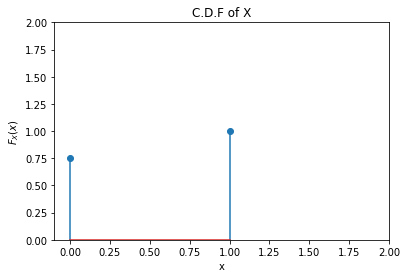
\includegraphics[width=8cm]{cdf_x.png}
    \caption{CDF of $X$}
    \label{Figure_1}
\end{figure}
\\
$F_Y(y)=
\begin{cases}
1, &y\geq1\\
\frac{1}{2}, & 0\leq y \leq1\\
0, &y<0
\end{cases}$

\begin{figure}[ht]
    \centering
    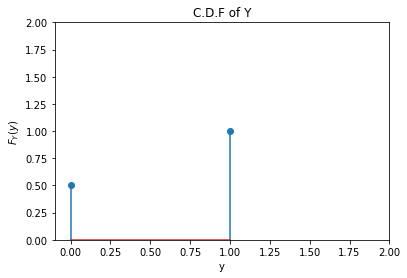
\includegraphics[width=8cm]{cdf_y.png}
    \caption{CDF of $Y$}
    \label{Figure_2}
\end{figure}

\begin{itemize}
    \item We can see that both $X$ and $Y$ are Bernoulli distributed.\\
    $\therefore$ Statement $\alpha$ is incorrect.\\
    \item Since $F_X(x)\neq F_Y(y)$, $X$ and $Y$ are not identically distributed.\\
    $\therefore$ Statement $\beta$ is incorrect.\\
    \item $\pr{X^2+Y^2=1}$
    \begin{align}
        &=\pr{X=0,Y=1}+\pr{X=1,Y=0}\nonumber\\
        &= \frac{1}{2}
    \end{align}
    $\therefore$ Statement $\gamma$ is correct.\\
    \item $\pr{XY=X^2Y^2}$
    \begin{align}
        &=\sum_{i=0}^1\sum_{j=0}^1\pr{X=i,Y=j}\nonumber\\
        &= 1
    \end{align}
    $\therefore$ Statement $\delta$ is correct.\\
\end{itemize}

$\therefore$ Option (d) is correct.

\end{document}